% Created 2022-02-23 Wed 11:52
% Intended LaTeX compiler: pdflatex
\documentclass[presentation,aspectratio=169]{beamer}
\usepackage[utf8]{inputenc}
\usepackage[T1]{fontenc}
\usepackage{graphicx}
\usepackage{grffile}
\usepackage{longtable}
\usepackage{wrapfig}
\usepackage{rotating}
\usepackage[normalem]{ulem}
\usepackage{amsmath}
\usepackage{textcomp}
\usepackage{amssymb}
\usepackage{capt-of}
\usepackage{hyperref}
\usepackage{khpreamble}
\usepackage{amssymb}
\usepgfplotslibrary{groupplots}
\newcommand*{\shift}{\ensuremath{\operatorname{q}}}
\usetheme{default}
\author{Kjartan Halvorsen}
\date{\today}
\title{Cinemática directa en 3D}
\hypersetup{
 pdfauthor={Kjartan Halvorsen},
 pdftitle={Cinemática directa en 3D},
 pdfkeywords={},
 pdfsubject={},
 pdfcreator={Emacs 26.3 (Org mode 9.4.6)}, 
 pdflang={English}}
\begin{document}

\maketitle

\section{Repetición}
\label{sec:org4b1e7bb}
\begin{frame}[label={sec:org23a0d08}]{Manipulador en 2D}
\begin{center}
 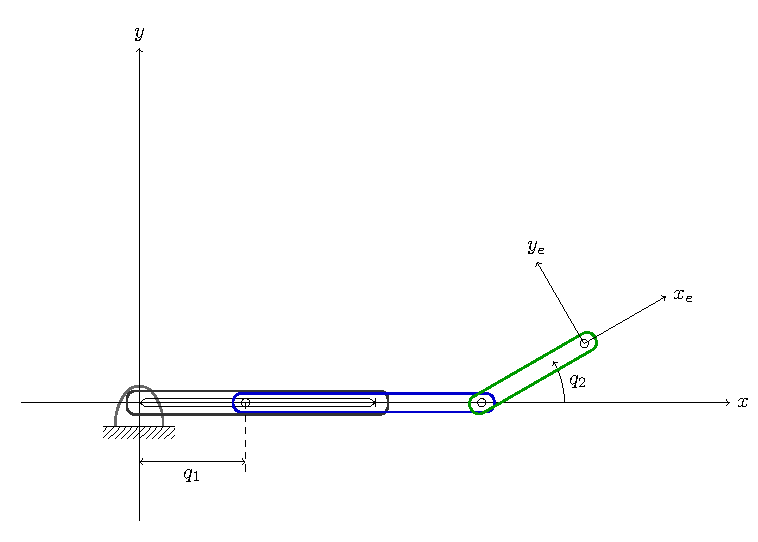
\includegraphics[height=0.8\textheight]{../figures/2d-2dof-prismatic-revolute.pdf}
\end{center}
\end{frame}

\section{Exponential map}
\label{sec:org2f5fd61}

\begin{frame}[label={sec:orgd94ebd3}]{Rotación sobre un eje}
\begin{center}
 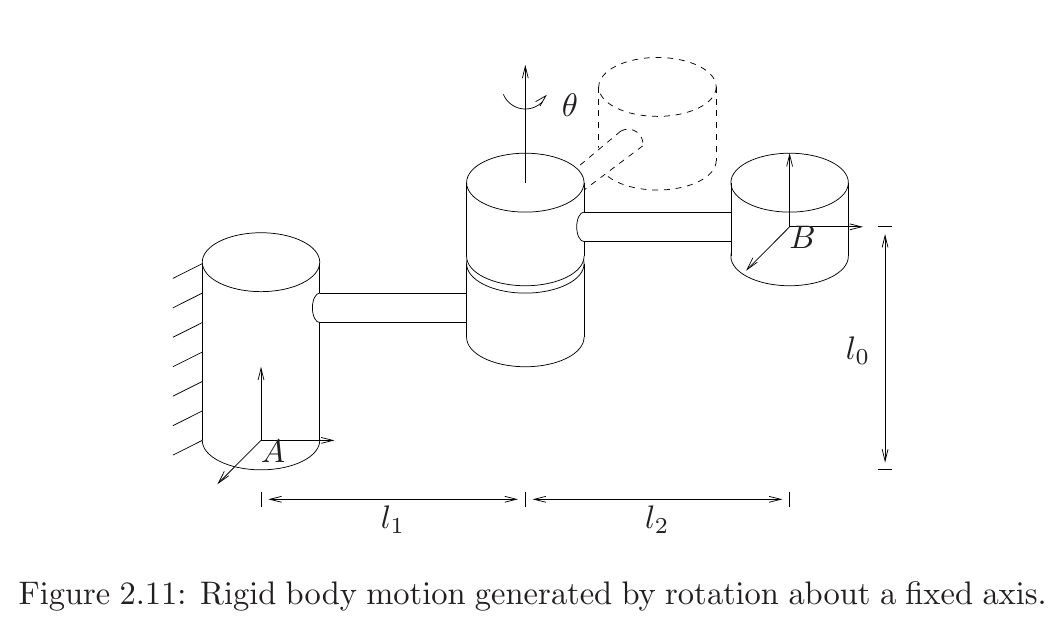
\includegraphics[height=0.8\textheight]{../figures/MLS-fig2.11.png}
\end{center}
\end{frame}


\begin{frame}[label={sec:org8e41adb}]{Manipulador en 3D}
\begin{center}
 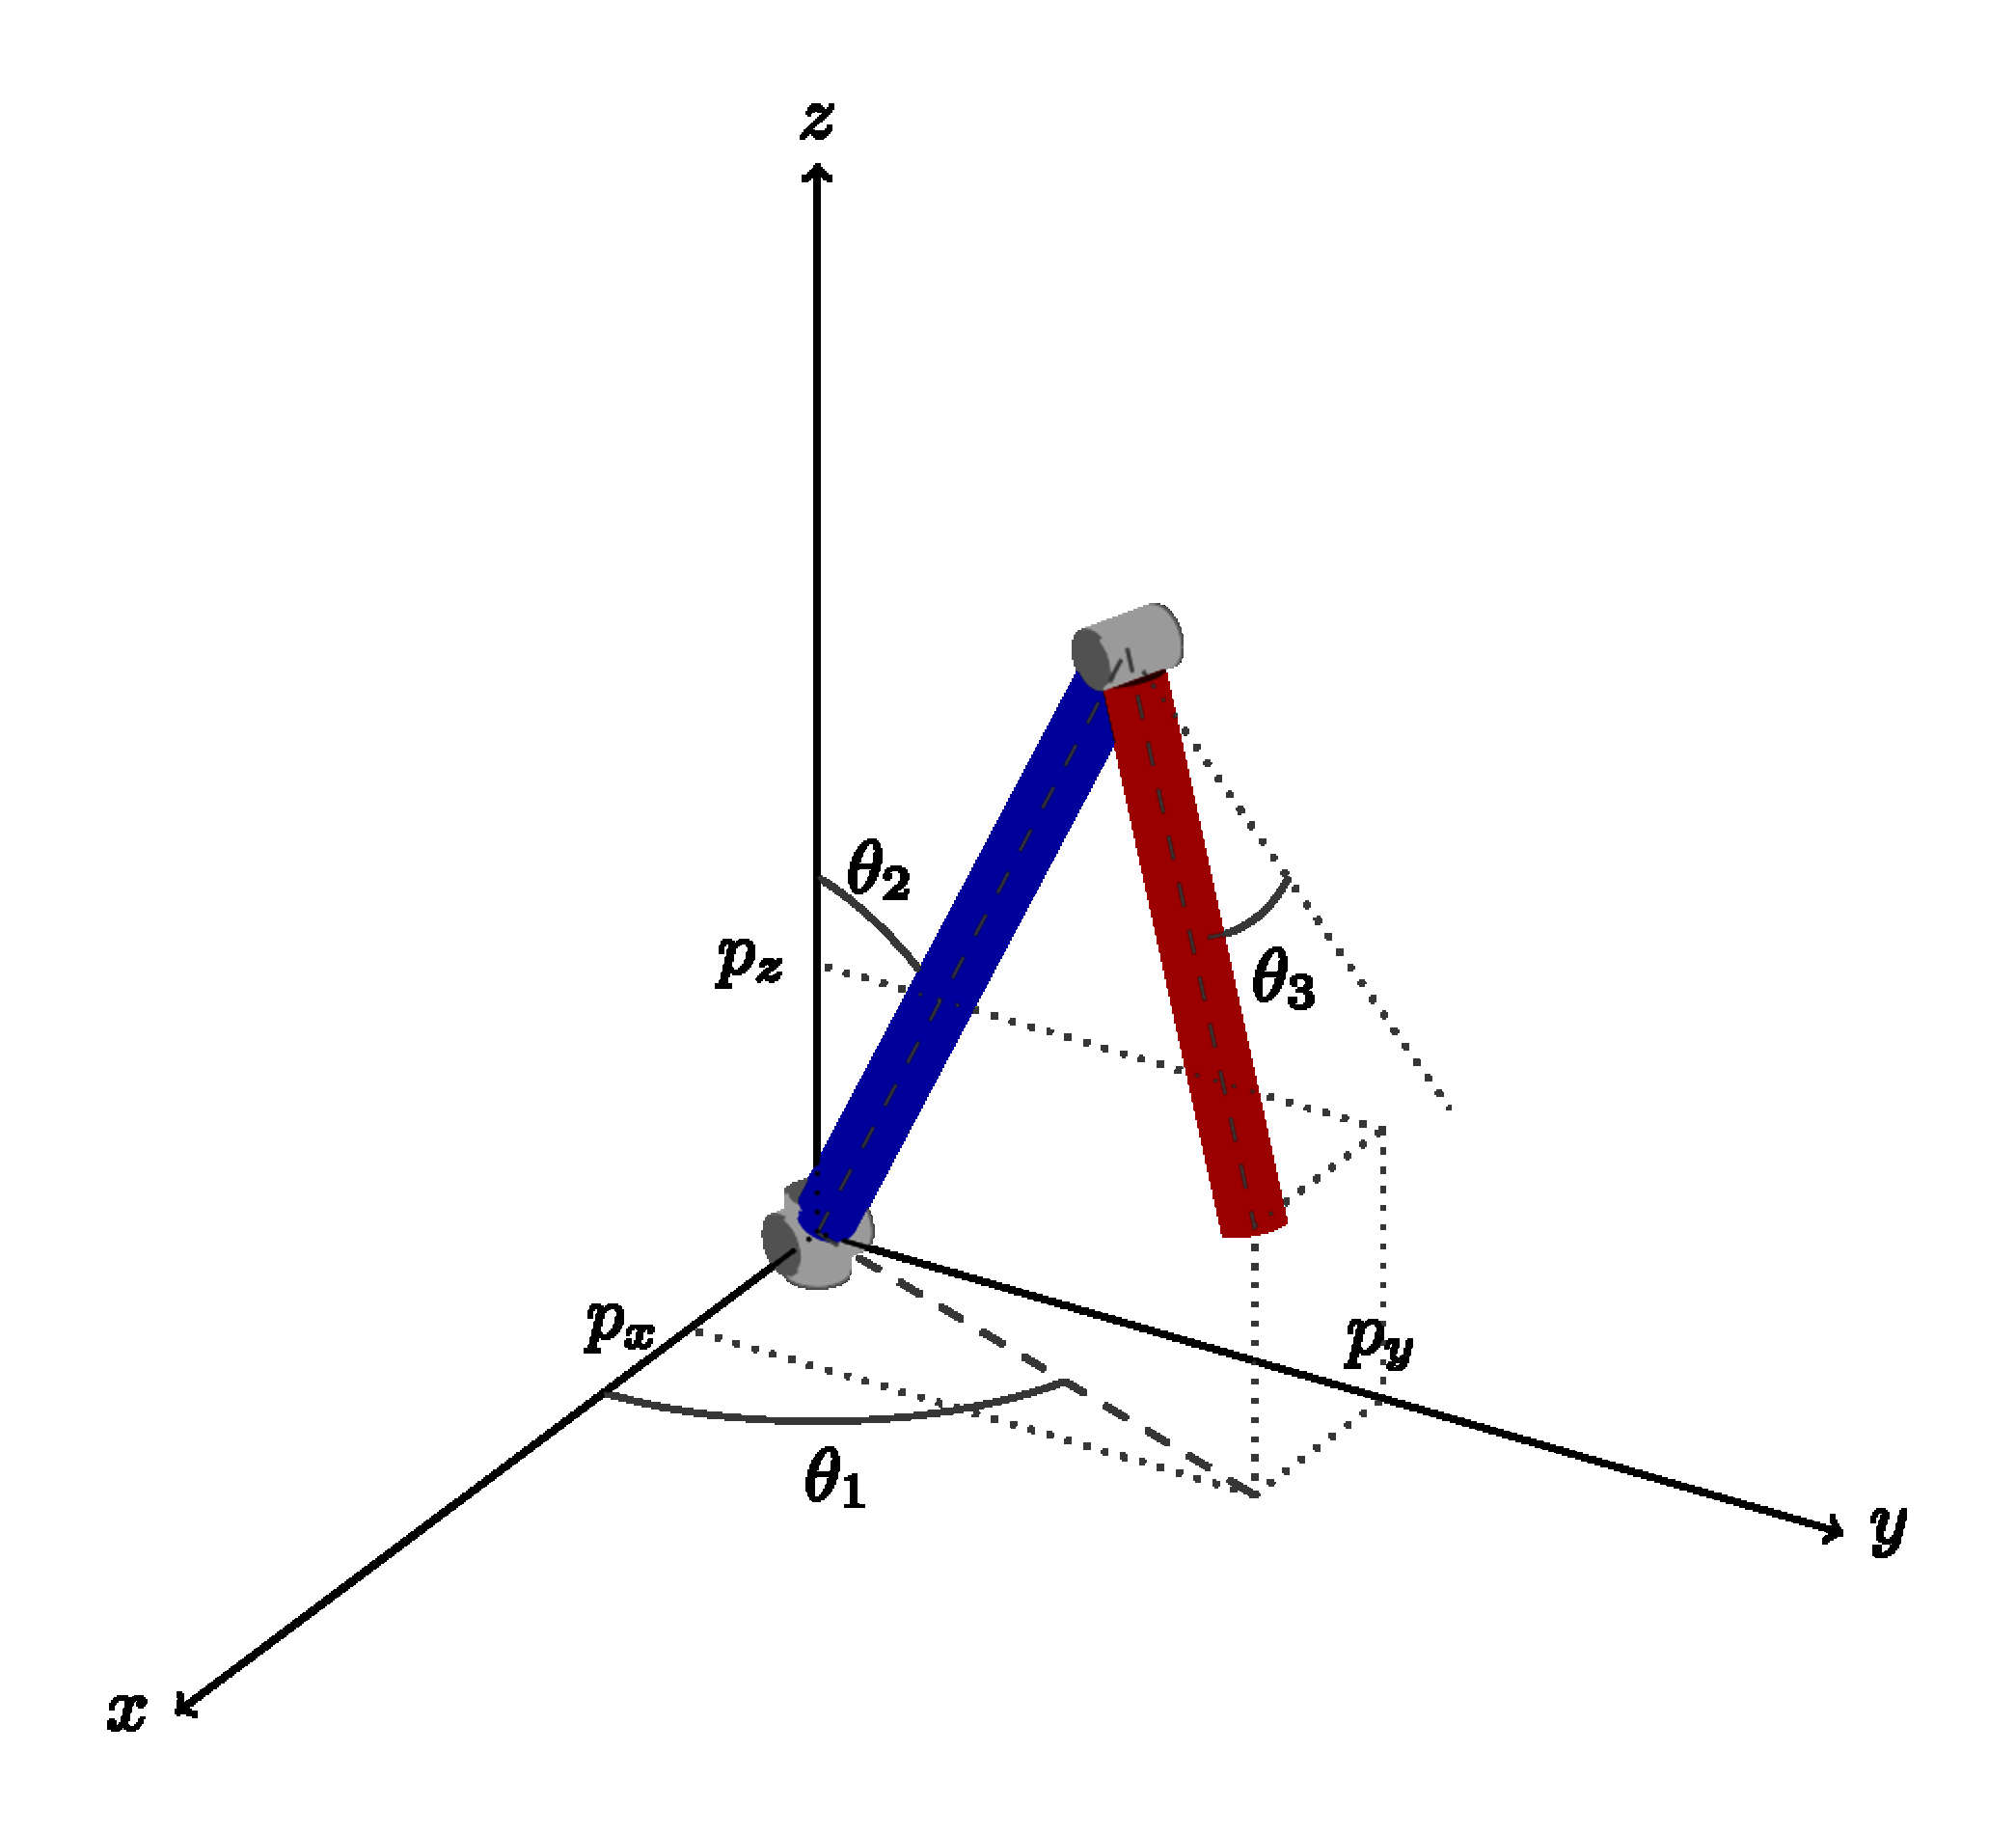
\includegraphics[height=0.8\textheight]{../figures/3d-3dof-revolute}
\end{center}
\end{frame}
\end{document}